%\textit{\textbf{The following section formatting is \textbf{optional}, you can also define sections as you deem fit.
%\\
%Focus on what future researchers or practitioners would find useful for reproducing or building upon the paper you choose.\\
%For more information of our previous challenges, refer to the editorials \cite{Sinha:2022,Sinha:2021,Sinha:2020,Pineau:2019}.
%}}
\section{Introduction}
\label{sec:intro}
%A few sentences placing the work in high-level context. Limit it to a few paragraphs at most; your report is on reproducing a piece of work, you don’t have to motivate that work.

% TODO: What problem the authors solve (motivation)
Tree-based models (TBM) are commonly used in machine learning.
The two most popular TBM are without doubt decision trees (CART)~\cite{breiman1984cart} and random forests (RF)~\cite{breiman2001random}.
The prior due to its simplicity is used to explain more complex model decisions, while the latter due to its robustness is used as a baseline for other models. 
Both models usually use the leaf sample average to make predictions. 
Agarwal et al~\cite{agarwal2022} argue that this approach is not necessarily optimal and propose a new post-hoc algorithm called Hierarchical Shrinkage (HS) where models instead make predictions based on the weighted average of the mean responses over the leaf and each of its ancestors.

% TODO: What did the authors do
The authors in~\cite{agarwal2022} first derive HS and compare it to other similar approaches: CART with cost-complexity pruning, C4.5~\cite{quinlan2014c4} (employes pruning during the creation of a tree), and GOSDT~\cite{pmlr-v119-lin20g} (limits search space during construction of a tree and is not greedy).
The authors evaluate HS on both CART and RF models, across both classification and regression each containing eight commonly used datasets.
In each test-case authors compare the TBM with HS and other regularization methods to assess whether HS improves the predictive power of the two most popular TBM and how it compares to other regularization algorithms in terms of speed and predictive improvement.

% TODO: What did we do
In our analysis, we used the Python library provided by Agarwal et al~\cite{agarwal2022} for the HS, while for other algorithms we used the libraries and models cited in the paper. Our analysis mainly focused on statistically quantifying whether and by how much HS improves the predictive power of CART and RF relative to other regularization methods. 

\section{Scope of reproducibility}
\label{sec:claims}

%The authors of the HS method state that their algorithm improves predictive performance of TBM on real-world datasets, and that the improvement is more significant for smaller datasets. Predictive performance curves are often U-shaped due to bias-variance tradeoff, but the authors claim that HS is able to reduce variance, which prevents overfitting.

The authors of the HS method make many claims about improving predictive performance over other methods and making more robust and simpler explanations. In this paper, we focused on the four claims we deemed most important:

\begin{itemize}
    \item \textbf{Claim 1: HS increases the predictive power of TBM.} \\ The authors claim that the use of HS can improve the predictive performance of TBM, such as CART and RF.
    \item \textbf{Claim 2: HS is better than other regularization algorithms for TBM.} \\ The authors claim that TBM with HS applied performs better than other regularization methods for TBM.
    \item \textbf{Claim 3: HS is faster than other regularization algorithms for TBM.} \\ The authors claim that HS is faster than other regularization methods for TBM because it does not make structural modifications to the TBM.
    \item \textbf{Claim 4: HS leads to more intuitive and robust explanations of RF.} \\ The authors claim that HS removes sampling artifacts and thus simplifies decision boundaries for RF and stabilizes feature importance, which makes it easier to interpret interactions in the model.
\end{itemize}

%For each claim, we decided to use specific metrics to evaluate its accuracy. We used metrics such as AUC/ROC and $ R^{2} $, and when comparing different methods, we used likelihood.

\mycomment{
For each claim made in the original paper, we devised a set of formal metrics to evaluate the accuracy of each claim.
Below we list the claims and the formal evaluation metrics used to verify each claim:

\begin{itemize}[label={}]
    \item \textbf{Claim 1: HS increases the predictive power of TBM}
    \vspace{-0.5em}
    \begin{itemize}[label={}, leftmargin=4.3em]
        \item[\textbf{Metrics}:] likelihood of HS improving the AUC/ROC or $R^2$ of DT, \\ % predictive power / predictions instead of AUC/ROC or $R^2$
                                likelihood of HS-DT achieving a higher AUC/ROC or $R^2$ than DT, \\
                                likelihood of HS improving the AUC/ROC or $R^2$ of RF, \\
                                likelihood of HS-RF achieving a higher AUC/ROC than RF.
    \end{itemize}
    \item \textbf{Claim 2: HS is better than other regularization algorithms for TBM}
    \vspace{-0.5em}
    \begin{itemize}[label={}, leftmargin=4.3em]
        \item[\textbf{Metrics}:] likelihood of HS-DT achieving a higher AUC/ROC or $R^2$ than DT-LBS, \\
                                likelihood of HS improving the AUC/ROC or $R^2$ of DT-CPP, \\
                                likelihood of HS-RF achieving a higher AUC/ROC than RF with tunned max depth ($d_{max}$) parameter, \\
                                likelihood of HS-RF achieving a higher AUC/ROC than RF with tunned max number of features used for tree splits ($mtry$).
    \end{itemize}
    \item \textbf{Claim 3: HS is faster than other post-hoc regularization algorithms for TBM}
    \vspace{-0.5em}
    \begin{itemize}[label={}, leftmargin=4.3em]
        \item[\textbf{Metrics}:] likelihood that HS-DT runtime is shorter than DT-CPP runtime evaluated using both (CPU and wall time), \\
                                 likelihood that HS-RF runtime is shorter than RF-$d_{max}$, RF-$d_{mtry}$ and BART runtime evaluated using both (CPU and wall time).
    \end{itemize}
    \item \textbf{Claim 4: HS leads to more intuitive and robust explanations of TBM (Domen)}
    \vspace{-0.5em}
    \begin{itemize}[label={}, leftmargin=4.3em]
        \item[\textbf{Metrics}:] HS simplifies decision boundaries of RF when using only two features, \\
                                 HS reduces the variance of shapley values, \\
                                 HS makes fitted function closer to being additive.
    \end{itemize}
\end{itemize}
}

% TODO: a couple of words on what we did and maybe what we improved (maybe - currently I am leaving it blank)

%\jdcomment{To organizers: I asked my students to connect the main claims and the experiments that supported them. For example, in this list above they could have ``Claim 1, which is supported by Experiment 1 in Figure 1.'' The benefit was that this caused the students to think about what their experiments were showing (as opposed to blindly rerunning each experiment and not considering how it fit into the overall story), but honestly it seemed hard for the students to understand what I was asking for.}

\section{Methodology}
%Explain your approach - did you use the author's code, or did you aim to re-implement the approach from the description in the paper? Summarize the resources (code, documentation, GPUs) that you used.

We used the Hierarchical Shrinkage predictors~\cite{agarwal2022} provided by the authors in the Python library {\sf imodels}\footnote{https://github.com/csinva/imodels}. We also used the provided {\sf get\_clean\_dataset} function to load all of the pre-cleaned datasets the authors used. In terms of code, our contribution lay in the setup and implementation of our claim-verifying experiments (Sec.~\ref{sec:results}) and the re-im\-ple\-men\-ta\-tion of the authors' notebooks which either did not run or did not return results consistent with the paper (Sec.~\ref{appendix}).

\subsection{Model descriptions}
%Include a description of each model or algorithm used. Be sure to list the type of model, the number of parameters, and other relevant info (e.g. if it's pretrained).

HS algorithm modifies the prediction values of the nodes for a TBM. HS transforms the prediction function of the TBM to

\begin{equation}
    \hat f_{\lambda}(x) = \mathbb{E}_{t_{0}}\{y\} + \sum_{l=1}^{L}\frac{\mathbb{E}_{t_{l}}\{y\}-\mathbb{E}_{t_{l-1}}\{y\}}{1+\frac{\lambda}{N(t_{l-1})}}
\end{equation}

where $ x $ is a query point, $ t_{0} $ denotes the root node, $ t_{l} $ denotes a node in the root-to-leaf path, $ \mathbb{E}_{t_{l}}\{y\} $ is the expected value of target variable at node $ t_{l} $, $ N(t_{l}) $ is the number of samples at node $ t_{l} $, and $ \lambda $ is a hyperparameter, either specified by the user or determined via cross-validation. The function can be seen as a weighted sum where more weight is given to the nodes that are closer to the root.

We used the CART algorithm to build decision trees and random forests. For specific claims, we used the C4.5 and GOSDT algorithms.

\subsection{Datasets}
%For each dataset include 1) relevant statistics such as the number of examples and label distributions, 2) details of train / dev / test splits, 3) an explanation of any preprocessing done, and 4) a link to download the data (if available).

We used the same datasets as the authors. The details can be found in Appendix~\ref{appendix:data}. We downloaded all of our datasets using the {\sf get\_clean\_dataset} function from the {\sf imodels} library. The data in the datasets were cleaned by the authors, therefore by using these datasets we ensured that we used the same pre-processing methods as the authors. We also checked each dataset, searched for them online in public databases, and compared them to the ones the authors provide. We were able to find all of the datasets and ensured that the ones we found are the same ones the authors provide. The only dataset we were unable to verify was German credit. The dataset we found has the same features, number of instances, and target variable distribution, but some of the features have slightly different value distributions. Despite this discrepancy, we proceeded to use the dataset, provided by the authors.

We used $2/3$ of our data for training and $1/3$ for testing. For tunning, we used 3-fold cross-validation using only samples from the training set. All splits were done randomly (for classification tasks we used stratified splits).

%For each claim, we decided to use specific metrics to evaluate its accuracy. We used metrics such as AUC/ROC and $ R^{2} $, and when comparing different methods, we used likelihood.
% TODO write metrics here?

\subsection{Hyperparameters}
% Describe how the hyperparameter values were set. (Y)
% The range of hyperparameters searched over. (Y)
% The method used to search. (Y)
% Best hyperparameter found. 
% Include the number of total experiments (e.g. hyperparameter trials). (Y)

For each experiment we performed several random splits; for each of the splits we found the best parameters with hyperparameter search (HPS). 
We always used the test metric as our objective function for HPS. 
In experiments, where the hyperparameter space was specified by the authors we used grid search, while in instances when it was not we used Bayesian optimization over a range of reasonable values. We performed grid search manually and we used the {\sf gp\_minimize()} function from {\sf scikit-optimize} for Bayesian optimization\footnote{For Bayesian optimization we used expected improvement as the evaluation function. We conducted 15 trials each with 5 initial starting points. The noise in our kernel was set to $\sigma=0.01$. We did not change other hyperparameters from their default values.}. 
We selected the HS regularization parameter with grid search from the set $\lambda_{HS} \in \left\{ 0.1, 1, 10, 25, 50, 100 \right\}$.
The same set of parameters was used in all instances where we applied HS post-hoc.
Additionally, when comparing HS-RF with other regularization methods we used Bayesian optimization to select the optimal maximum depth of our RF trees from the range $d_{max} \in (1, 30)$, as well as the best fraction of features used when splitting a RF tree from the range $mtry \in (0.1, 1.0)$.
These two post-hoc regularization methods were applied separately following the original paper.
For the cost-complexity pruning (CCP) $\alpha$ parameter we used the approach from the original paper where $\alpha$ is chosen for each cross-validation fold from the $\alpha$ returned by {\sf scikit-learn.cost\_complexity\_pruning\_path} such that the number of leaves in the prunned DT is as close as possible to the specified number of leaves.
Additionally, during our HPS we analyzed the sensitivity of our results to shifts in each individual parameter.
We found that increasing regularization for HS-DT and HS-CCP lead to significantly poorer performance for both regularization and classification, while for HS-RF it had the opposite effect improving the models' performance.
For HS-RF the number of trees used did not appear to be correlated with the performance of the model indicating that we could have used a smaller number of trees to achieve similar results. This was not the case for DT where increasing the number of leaves lead to a significant improvement in performance.



\subsection{Experimental setup and code}
%Include a description of how the experiments were set up that's clear enough a reader could replicate the setup. Include a description of the specific measure used to evaluate the experiments (e.g. accuracy, precision@K, BLEU score, etc.).  Provide a link to your code.

To perform our experiments we used the authors' code from their Python package {\sf imodels} for applying HS and reading datasets and our code. We used Python 3.10 and libraries {\sf NumPy, pandas, scikit-learn, matpotlib, plotnine}, and others. We structured our experiments into Jupyter notebooks, one notebook per claim.

% TODO
% describe the setup for individual claims

We also tested the validity of their HS implementation by building deterministic trees with CART and manually calculating the application of HS. The tests are in folder {\sf tests}. One tests the HS on regressive tasks and the other on classification tasks.

The metrics the authors and we use are the area under the curve (AUC/ROC) for classification and $ R^{2} $ for regression. We take both from the {\sf scikit-learn} library. For the improvement comparison, we used the region of practical equivalence of 0.005.

% TODO link to our code

\subsection{Computational requirements}
% Include a description of the hardware used, such as the GPU or CPU the experiments were run on. 
We ran our experiments on two computers with the following two CPUs: Intel(R) Core (TM) i7-9750H CPU @2.60GHz ($\text{CPU}_1$) and AMD Ryzen 5 5600X 6-Core ($\text{CPU}_2$).
Comparing CART with HS-CART for classification took 37 minutes (100 repeats) while performing a similar experiment comparing CCP (100 repeats) with HS took 4 hours. Measurements were done in wall time.
Comparing RF with other regularization methods on classification datasets took roughly 4.5 hours.
For DT cpu and wall time are almost identical, while for RF the cpu time is roughly $50\%$ larger than wall time.
Classification and regression for claims 1, 2, and 3 were run on $\text{CPU}_2$, with the exception of LBS for claim 2 which we ran on $\text{CPU}_1$.
All experiments for claim 4 were run on $\text{CPU}_1$.

% Generally, consider the perspective of a reader who wants to use the approach described in the paper --- list what they would find useful.

\section{Results}
\label{sec:results}

Our results show that HS improves DT scores and is one of the best forms of regularization in comparison to other DT regularization methods both in terms of predictive power as well as in terms of speed. 
Our results do not indicate that HS is better for RF than other regularization methods in terms of predictive power, however, they do show that HS is significantly faster than other regularization methods and is easier to interpret.

%\subsection{Results reproducing original paper}
% For each experiment, say 1) which claim in Section~\ref{sec:claims} it supports, and 2) if it successfully reproduced the associated experiment in the original paper. 
% For example, an experiment training and evaluating a model on a dataset may support a claim that that model outperforms some baseline.
% Logically group related results into sections. 

%\subsection{Claim 1: HS increases the predictive power of TBM.}

% TODO
% likelihood of HS improving the AUC/ROC or R2 of RF,
% likelihood of HS-RF achieving a higher AUC/ROC than RF
% put miscelenious claims somewere (maybe)
% briefly explain Bayesian model used to get results

\begin{figure}[hbt]
     \centering
     \begin{subfigure}[b]{0.43\textwidth}
         \centering
         \includegraphics[width=\textwidth]{images/claim1/any-dt.png}
         \caption{Likelihood of improvement for DT.}
         \label{fig:claim1-dt}
     \end{subfigure}
     \hfill
     \begin{subfigure}[b]{0.43\textwidth}
         \centering
         \includegraphics[width=\textwidth]{images/claim1/any-rf.png}
         \caption{Likelihood of improvement for RF.}
         \label{fig:claim1-rf}
     \end{subfigure}
        \caption{This set of images shows the likelihood that HS improves a TBM score. 
        For DT, the likelihood of improvement is the highest, while for RF the likelihood of no change is the highest.}
        \label{fig:claim1-improvement}
\end{figure}

\begin{figure}[hbt]
     \centering
     \begin{subfigure}[b]{0.43\textwidth}
         \centering
         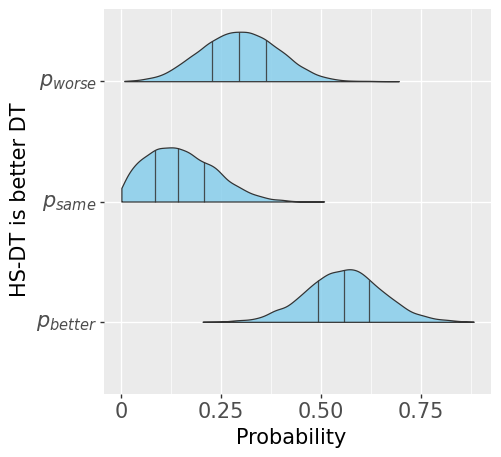
\includegraphics[width=\textwidth]{images/claim1/rnd-dt.png}
         \caption{Likelihood that HS-DT is better than DT.}
         \label{fig:claim1-rnd-dt}
     \end{subfigure}
     \hfill
     \begin{subfigure}[b]{0.43\textwidth}
         \centering
         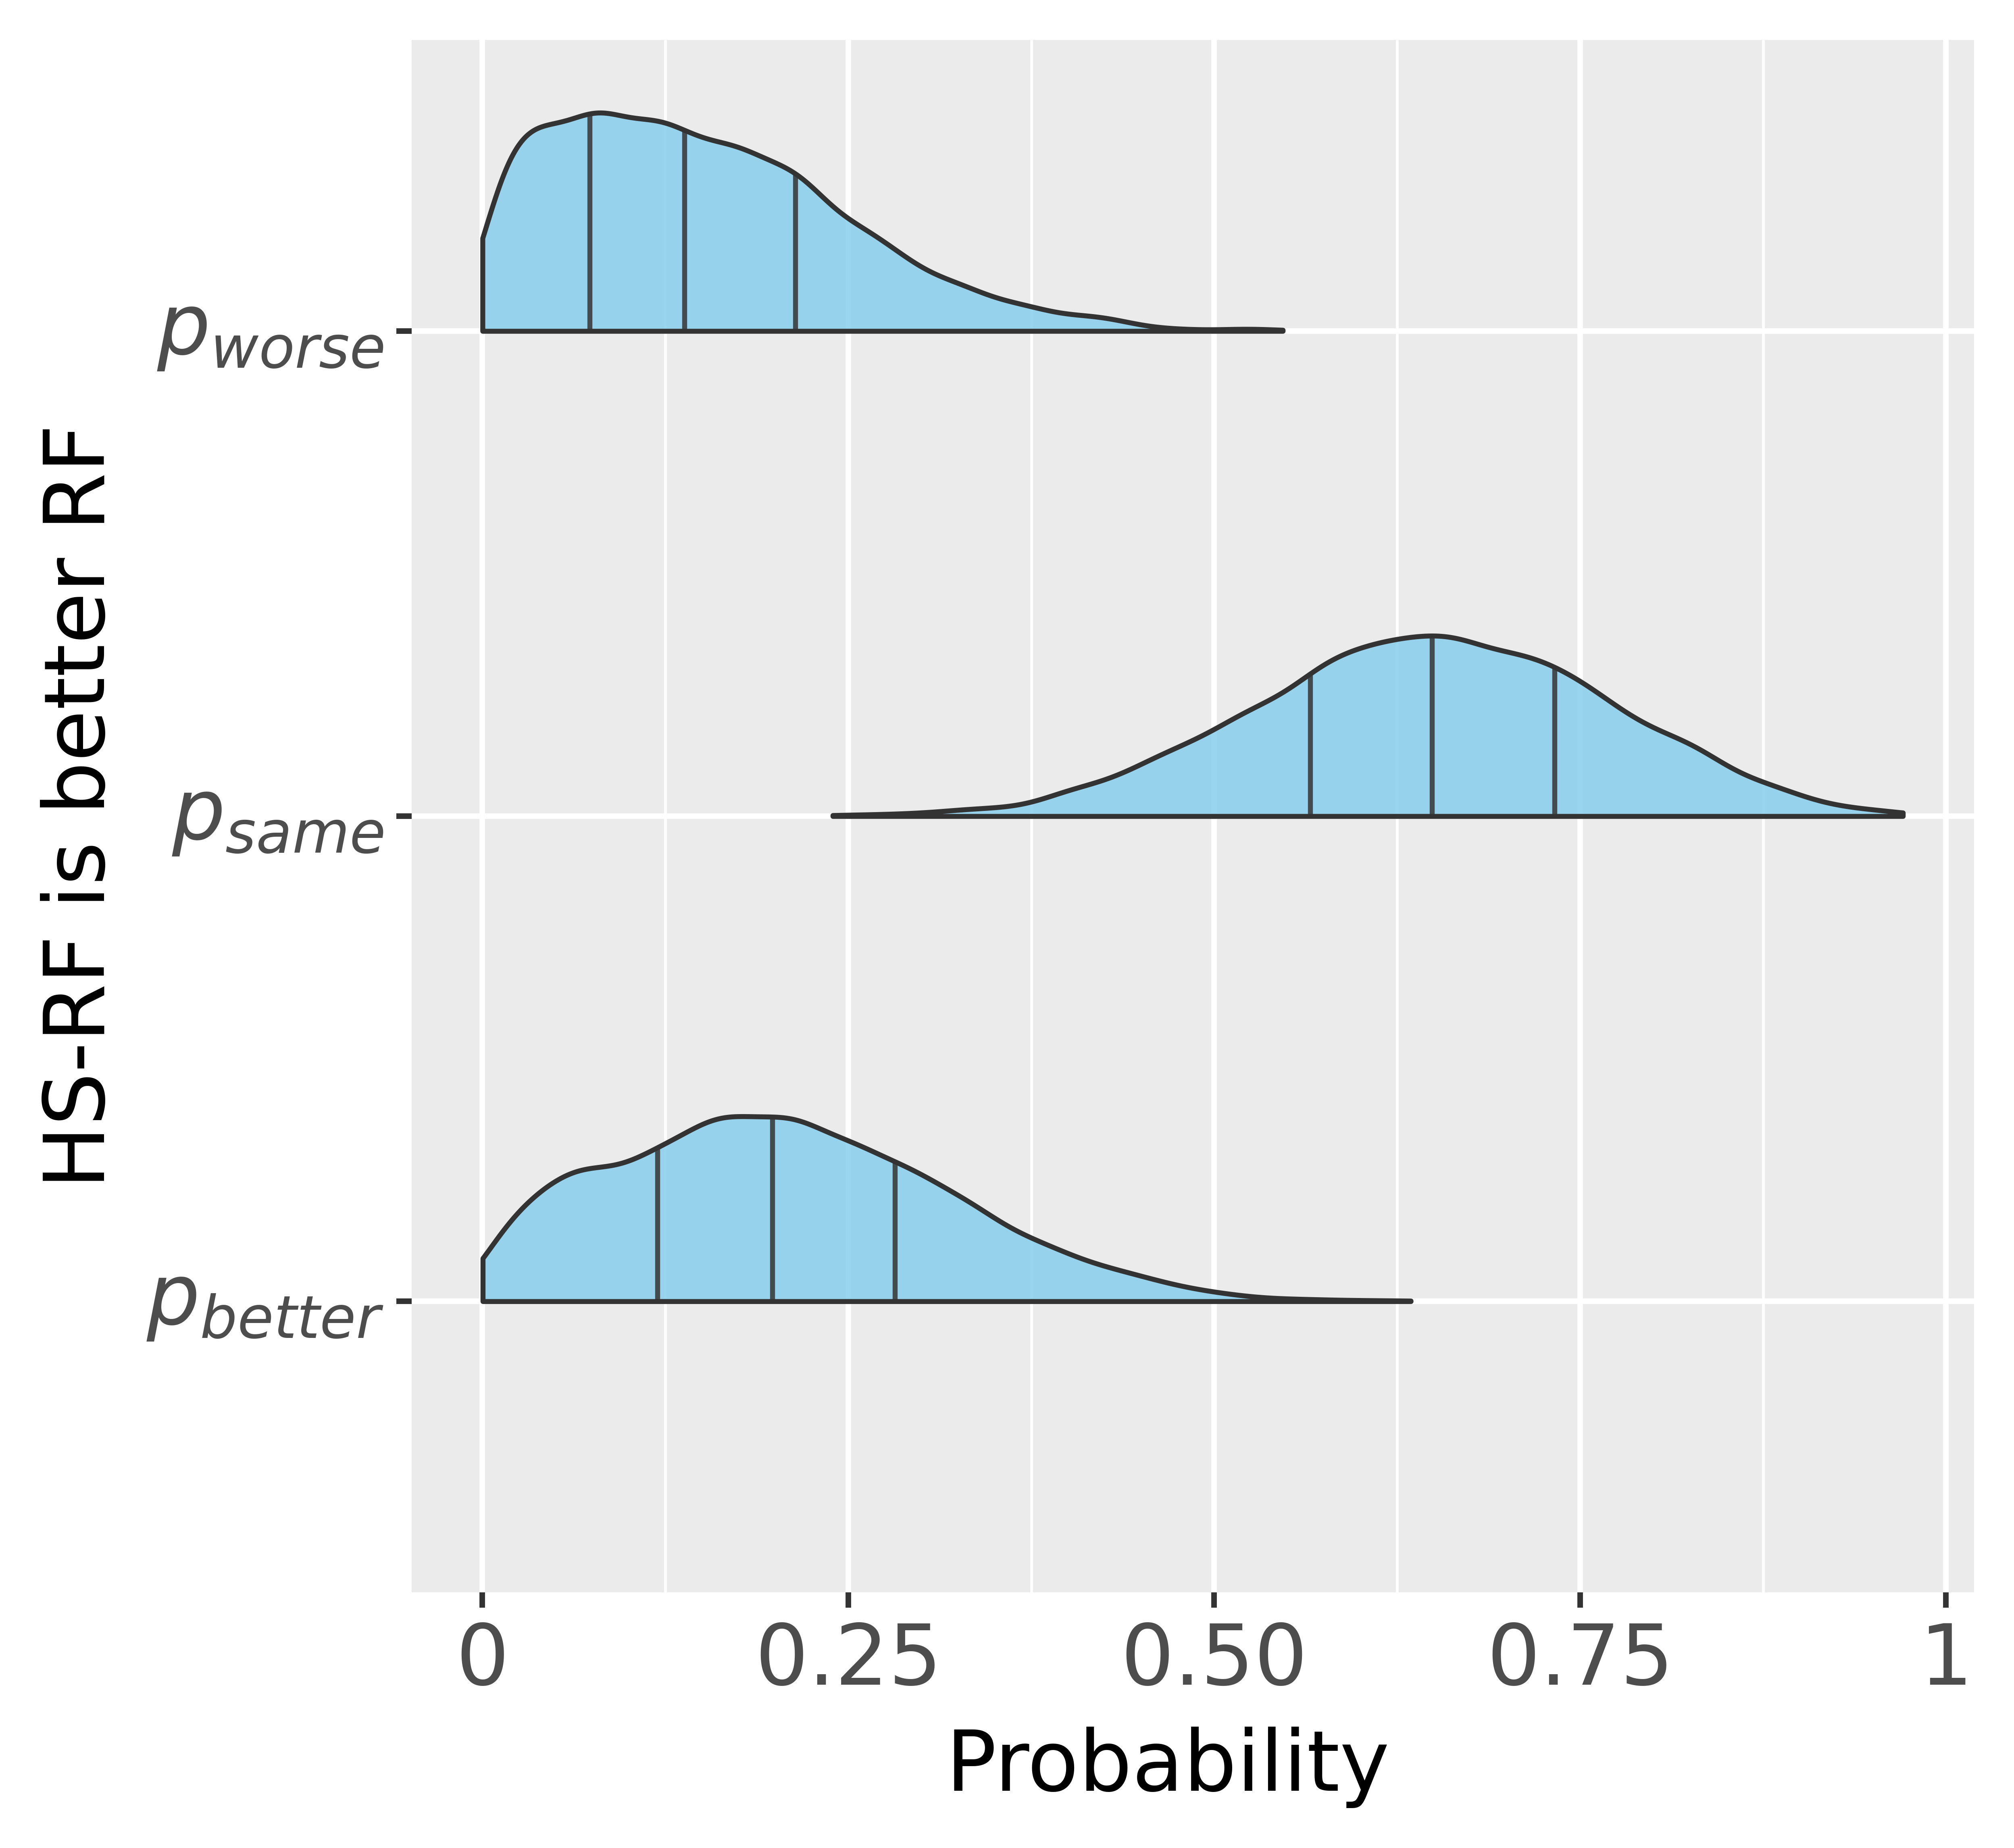
\includegraphics[width=\textwidth]{images/claim1/rnd-rf.png}
         \caption{Likelihood that HS-RF is better than RF.}
         \label{fig:claim1-rnd-rf}
     \end{subfigure}
        \caption{This set of images shows the likelihood that a TBM with HS is better than one without HS. 
        There is a significant likelihood of HS-DT being better than DT, while there is no significant likelihood that HS-RF will be better than RF.}
        \label{fig:claim1-better}
\end{figure}

\subsection{Claim 1: HS increases the predictive power of TBM.}

The authors claim that applying HS to TBM significantly improves their prediction performance. 
They test this by applying HS to DT and RF across 16 different datasets; authors vary the maximum number of leaves for DT and the maximum number of trees for RF to test how HS improves TBM when the complexity of the models changes.
The authors evaluate the results using several metrics, though they mainly focus on AUC/ROC for classification and $R^2$ for regression.

We split the author's claim that HS improves the predictive power of TBM into the likelihood that HS improves the model it is applied to (Fig.~\ref{fig:claim1-improvement}) and the likelihood that HS applied to a TBM on average gives better results (Fig.~\ref{fig:claim1-better}). 
The authors mix these two claims thereby summing together the variance of TBM with the variance of the improvement resulting from HS, as such their results do not conclusively corroborate either of the claims.

To analyze whether HS improved a specific TBM we created a categorical variable that represented whether HS improved the score of the TBM. We then fit a hierarchical categorical model\footnote{\label{fn:prior} We used the same normal prior $p_i[d] \sim N(1/n, 0.5)$, where $p_i[d]$ is the probability of the event being in category $i$, $n$ is the number of categories and $d$ is the samples dataset.}, where the first level represented the dataset, and the category in the second level was whether applying HS improves our TBM score.

To analyze whether HS-TBM was on average better than TBM, we split our test scores into groups where each group was comprised of test scores from runs on the same dataset and the same number of leaves or trees, then for each model we randomly with replacement sampled 1000 instances using each regularization method and saved how HS-TBM fared in comparison to TBM. We then fit a hierarchical Categorical model\ref{fn:prior}, where the first level represented the dataset, and the category in the second level was how HS-TBM fared in comparison to TBM.

Our results (Fig.~\ref{fig:claim1-improvement}) confirm the sub-claim that by applying HS to the DT the score is likely to increase, however, this does not apply to RF with the likelihood of the score not changing being larger than $50\%$. 
Our results (Fig.~\ref{fig:claim1-better}) confirm the sub-claim that the likelihood of an HS-DT score is on average significantly better than a DT score (Fig.~\ref{fig:claim1-rnd-dt}), however, they do not confirm the sub-claim that HS-RF is on average better than RF (Fig.~\ref{fig:claim1-rnd-rf}), with a likelihood of over $60\%$ that there is no significant difference between HS-RF and RF. More detailed results are in Appendix~\ref{appendix:claim1}.

\subsection{Claim 2: HS is better than other regularization algorithms for TBM.}

The authors claim that DT with HS regularization achieves better results than DT with CCP or LBS regularization and that RF with HS regularization achieves better results than RF with $mtry$ or $d_{max}$ hyperparameter tunning. The authors use the same evaluation metrics as in Claim 1. For each dataset, the authors train all three TBM ten times and then evaluate it with AUC/ROC or $R^2$.

\begin{figure}[hbt]
     \centering
     \begin{subfigure}[b]{0.43\textwidth}
         \centering
         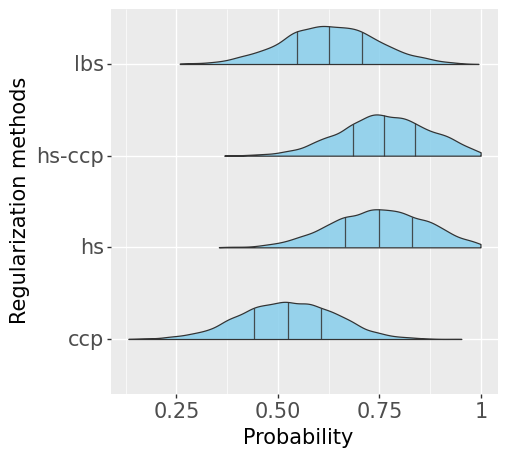
\includegraphics[width=\textwidth]{images/claim2/reg-dt.png}
         \caption{Likelihood of regularized DT achieving the best score}
         \label{fig:claim2-reg-dt}
     \end{subfigure}
     \hfill
     \begin{subfigure}[b]{0.43\textwidth}
         \centering
         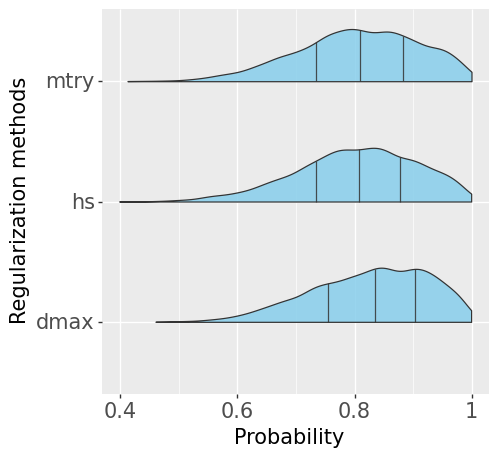
\includegraphics[width=\textwidth]{images/claim2/reg-rf.png}
         \caption{Likelihood of regularized RF achieving the best score}
         \label{fig:claim2-reg-rf}
     \end{subfigure}
        \caption{This set of images shows the likelihood that TBM regularized with a certain regularization method achieves the best score. 
        For DT HS is the best regularizer, significantly outperforming CCP and LBS.
        For RF all three method scores are almost indistinguishable.}
        \label{fig:claim2}
\end{figure}

We split our test scores into groups where each group was comprised of test scores from runs on the same dataset and the same number of leaves or trees, then for each model we randomly with replacement sampled 1000 instances using each regularization method and saved whether the method achieved the best results. Finally, we fit a hierarchical Bernoulli model$^{\ref{fn:prior}}$, where the first level represented the dataset, and the category in the second level was whether the model was the best or not.

Our results (Fig.~\ref{fig:claim2}) confirm the author's claim that HS is a better regularizer than CCP or LBS, with both HS-CCP and HS performing similarly indicating we are unlikely to significantly improve our results by combining HS and CCP.
Our results however do not confirm that HS is a better regularizer for RF compared to $mtry$ or $d_{max}$, with both methods performing similarly to HS.  More detailed results are in Appendix~\ref{appendix:claim2}.

\subsection{Claim 3: HS is faster than other post-hoc regularization algorithms for TBM.}

The authors claim that HS is faster than other post-hoc regularization algorithms for TBM.
The authors did not specify what experiments they conducted to verify this claim, however, we assumed the authors measured the wall and/or CPU time necessary to tune, train and test each model.

To check this claim, we measured both the CPU and wall time for the tunning, training and testing phase of each regularization algorithm for each dataset.
We summed the three phases together and calculated the difference between the mean times of HS and other regularization methods (Tab.~\ref{tab:claim3}).

Our results confirm the claim that HS is significantly faster in CPU time in comparison to all other regularization methods. 
While HS is also better in wall time the improvement is less pronounced.
The only instance where HS is slower than all other regularization methods is in the case of the Recidivism dataset. 
Considering this is true when comparing HS to both other regularization methods we consider this difference significant. Comparison of time complexity of different DT regularizers is in Appendix~\ref{appendix:claim3}.

\begin{table}[hbt]
    \centering
    \begin{tabular}{|l|c|rr|c|rr|}
    %\toprule
    %{} & \multicolumn{4}{|c|}{RF} %& \multicolumn{1}{2}{DT} \\
    \toprule
    {} & base & \multicolumn{2}{|c|}{overtime} & base & \multicolumn{2}{|c|}{overtime} \\
    \toprule
    {} &  \makecell{$hs$\\wall} & \makecell{$mtry$\\wall} &  \makecell{$d_{max}$\\wall} &  \makecell{$hs$\\cpu} &  \makecell{$mtry$\\cpu} &  \makecell{$d_{max}$\\cpu} \\
    dataset       &   {} & {} &        &           &            &           \\
    \midrule
    Heart         &    $3$ &    \cellcolor{blue!15}$2 \pm 1$ &        \cellcolor{blue!15}$2 \pm \,\,1$ & $3$  &   \cellcolor{blue!15}$11 \pm \,\,\,1$ &      \cellcolor{blue!15}$11 \pm \,\,\,1$ \\
    Breast cancer &    $4$ &    \cellcolor{blue!15}$2 \pm 1$  &        \cellcolor{blue!15}$2 \pm \,\,1$ & $4$ &    \cellcolor{blue!15}$10 \pm \,\,\,1$ &    \cellcolor{blue!15}$11 \pm \,\,\,1$  \\
    Haberman      &   $4$ &     \cellcolor{blue!15}$2 \pm 1$  &        \cellcolor{blue!15}$2 \pm \,\,1$ & $4$ &    \cellcolor{blue!15}$11 \pm \,\,\,1$ &      \cellcolor{blue!15}$11 \pm \,\,\,1$ \\
    Ionosphere    &    $3$ &    \cellcolor{blue!15}$3 \pm 1$ &        \cellcolor{blue!15}$4 \pm \,\,1$ & $3$ &    \cellcolor{blue!15}$12 \pm \,\,\,1$  &      \cellcolor{blue!15}$13 \pm \,\,\,1$ \\
    Diabetes      &    $5$ &   \cellcolor{gray!10}$1 \pm 1$  &        \cellcolor{blue!15}$2 \pm \,\,1$ &  $5$ &   \cellcolor{blue!15}$10 \pm \,\,\,1$ &      \cellcolor{blue!15}$10 \pm \,\,\,1$ \\
    German credit &    $6$ &   \cellcolor{gray!10}$0 \pm 1$  &        \cellcolor{gray!10}$1 \pm \,\,1$ & $6$ &     \cellcolor{blue!15}$9 \pm \,\,\,1$ &       \cellcolor{blue!15}$10 \pm \,\,\,1$ \\
    Juvenile      &    $12$ &   \cellcolor{red!15}$-2 \pm 5$ &       \cellcolor{blue!15}$23 \pm 2$ & $12$   &   \cellcolor{blue!15}$7 \pm 5$ &      \cellcolor{blue!15}$31 \pm 2$  \\
    Recidivism    &   $43$ &   \cellcolor{red!15}$-33 \pm 6$ &      \cellcolor{red!15}$-24 \pm 6$ &  $43$ &  \cellcolor{red!15}$-24 \pm 6$ &     \cellcolor{red!15}$-16 \pm 6$  \\
    \bottomrule
    \end{tabular}
    \caption{Average execution overtime ($\pm$ stderr) in seconds of regularized RF relative to HS-RF for classification. Blue indicates HS-RF was faster, red indicates it was slower and grey indicates the difference in mean execution times was smaller than the standard error of the difference.}
    \label{tab:claim3}
\end{table}

\subsection{Claim 4: HS leads to more intuitive and robust explanations of RF.}

The authors state that applying HS to RF removes sampling artefacts and simplifies decision boundaries. They test this by building an RF with 50 trees on only two of the most important features, determined by the mean decrease in impurity (MDI, Gini index).

Our results (Fig.~\ref{fig:claim4-boundary}) show that the boundaries are smoother after applying HS. HS prevents overfitting and therefore smoothes the boundary between the target classes. With simpler boundaries the model predictions can be better explained, leaving much less uncertainty. The boundaries for all of the classification datasets are in Appendix~\ref{appendix:claim4-decision}.

\begin{figure}[hbt]
    \centering
    \begin{subfigure}[b]{0.45\textwidth}
        \centering
        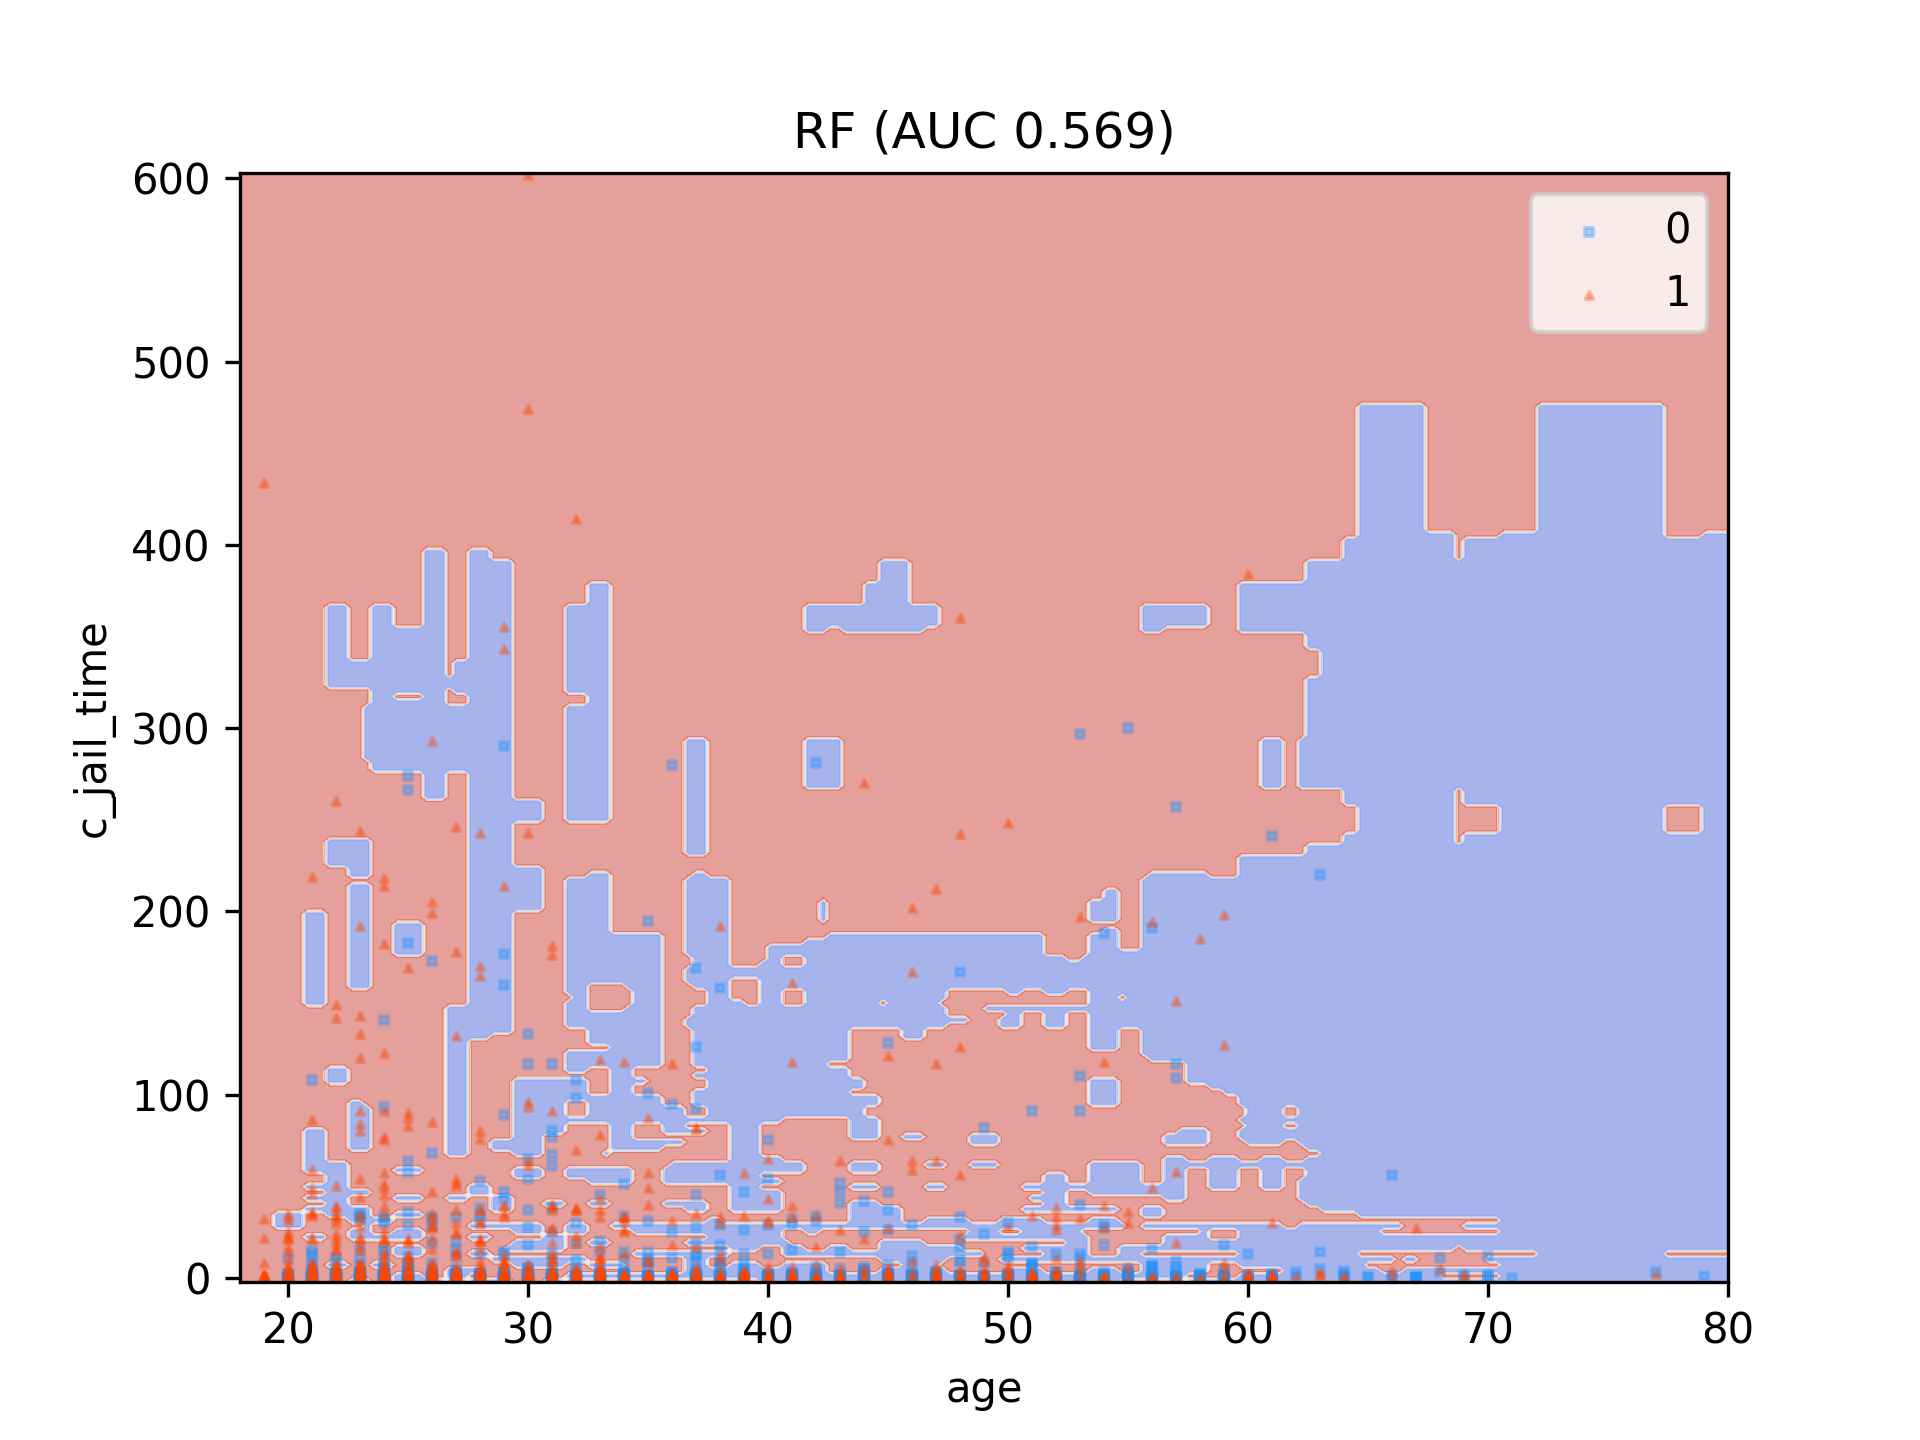
\includegraphics[width=\textwidth]{images/claim4/compas_two_year_clean_RF_reproduced.png}
        \caption{Recidivism RF \\ (AUC 0.569)}
        \label{fig:rrf}
    \end{subfigure}
    \begin{subfigure}[b]{0.45\textwidth}
        \centering
        \includegraphics[width=\textwidth]{images/claim4/compas_two_year_clean_hsRF_reproduced.png}
        \caption{Recidivism hsRF \\ (AUC 0.606)}
        \label{fig:rhsrf}
    \end{subfigure}

%    \begin{subfigure}[b]{0.45\textwidth}
%        \centering
%        \includegraphics[width=\textwidth]{images/claim4/german_RF_reproduced.png}
%        \caption{German credit RF \\ (AUC 0.594)}
%        \label{fig:gcrf}
%    \end{subfigure}
%    \begin{subfigure}[b]{0.45\textwidth}
%        \centering
%        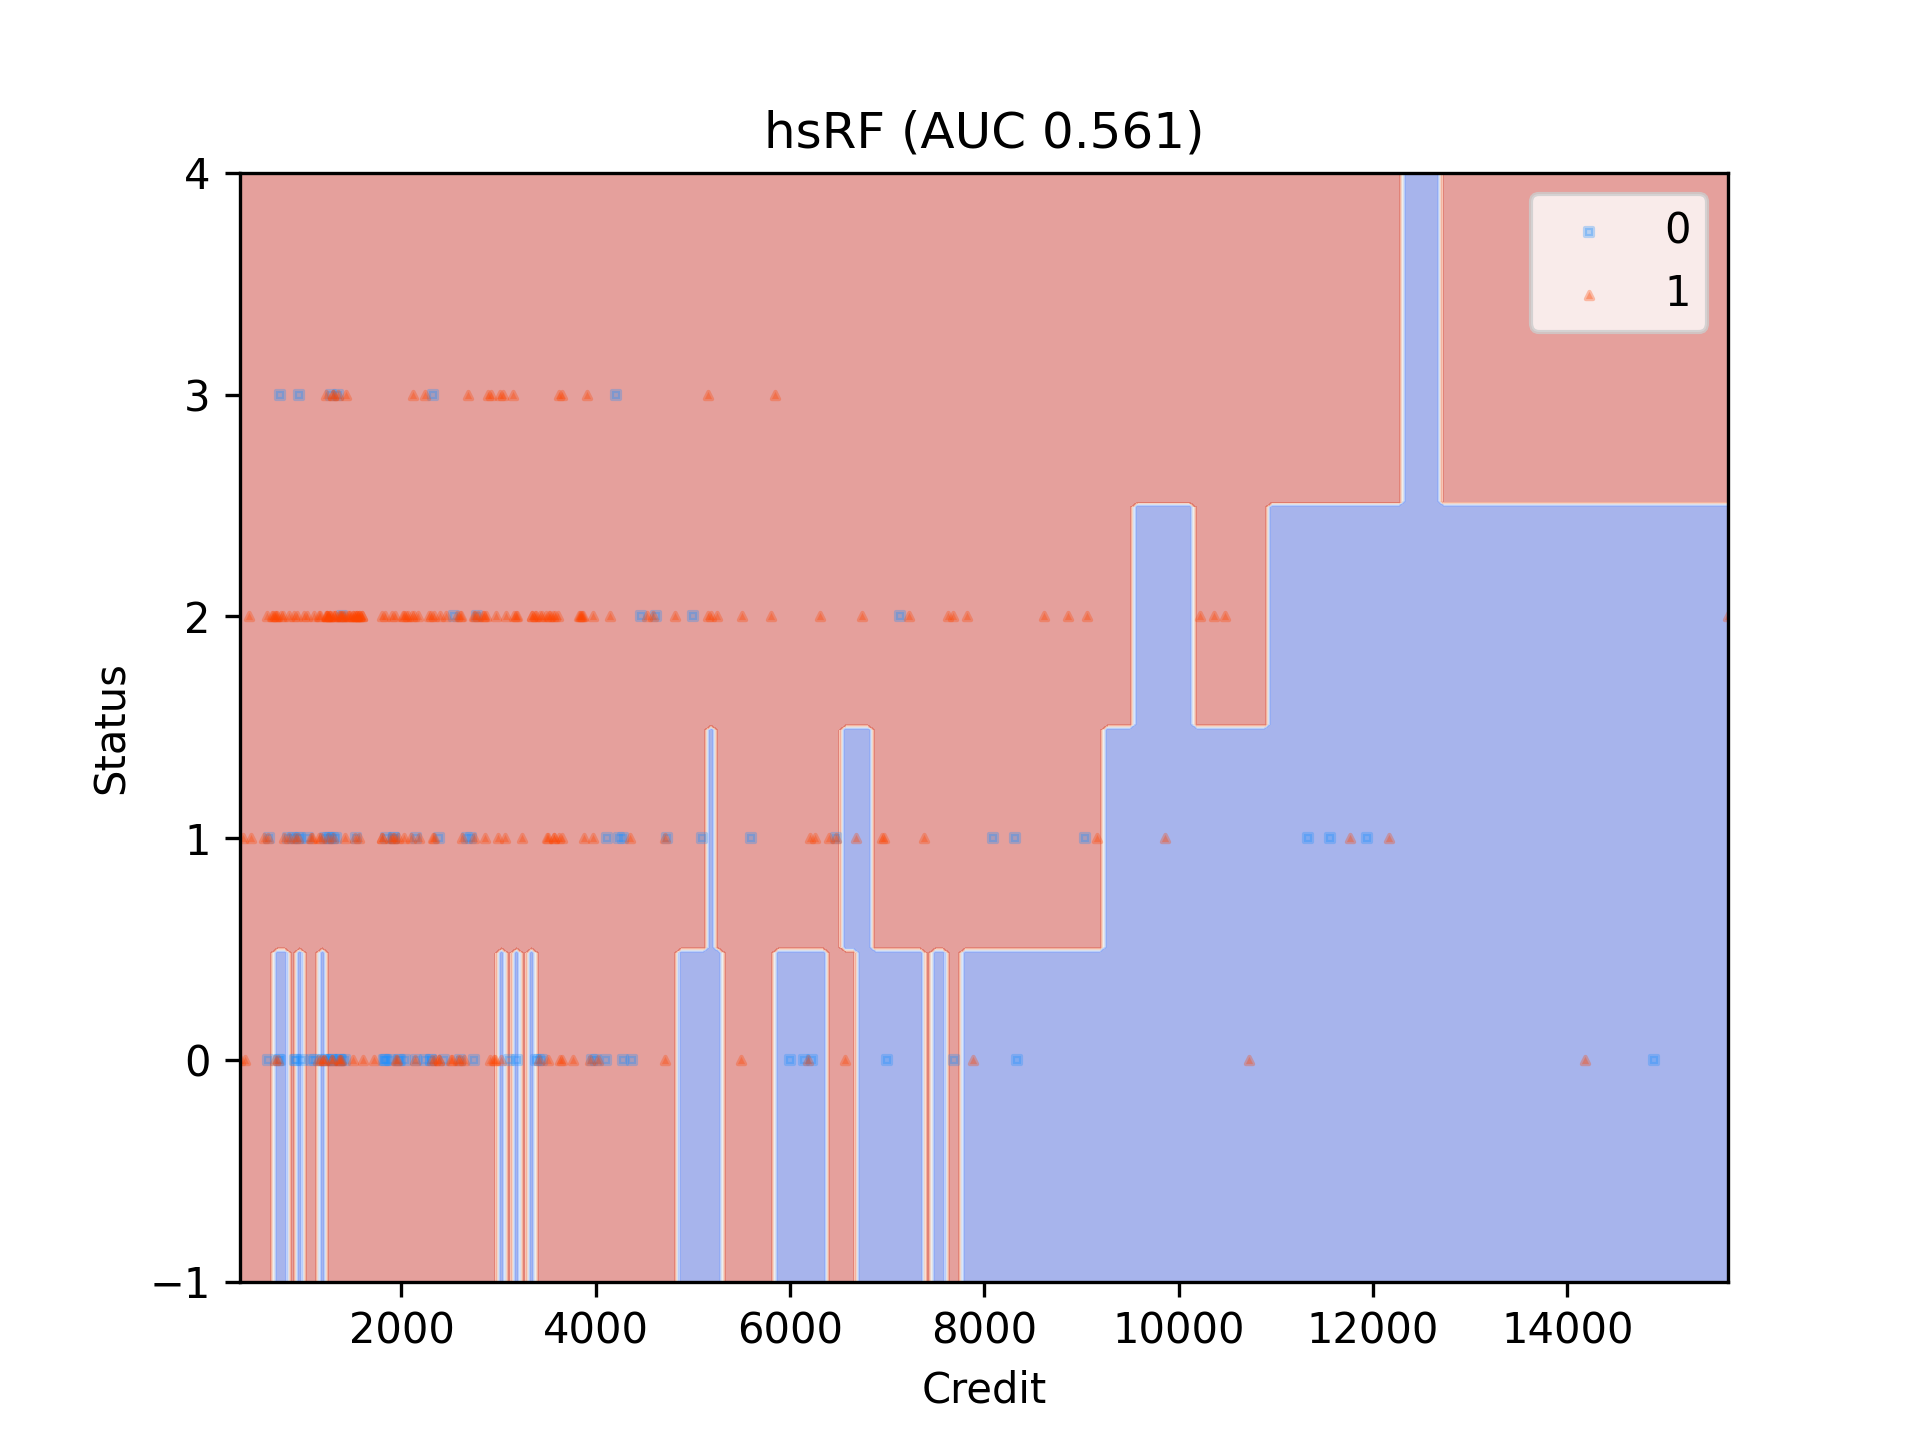
\includegraphics[width=\textwidth]{images/claim4/german_hsRF_reproduced.png}
%        \caption{German credit hsRF \\ (AUC 0.561)}
%        \label{fig:gchsrf}
%    \end{subfigure}
    \caption{Applying HS to RF simplifies boundaries. We have the decision boundary before (\ref{fig:rrf}) and after (\ref{fig:rhsrf}) applying HS on the Recidivism dataset on the two most important features, age and c\_jail\_time. % On the right, we have the decision boundary before (\ref{fig:gcrf}) and after (\ref{fig:gchsrf}) applying HS on the German credit dataset. The AUC in the first case improves, while in the second case worsens.
    }
    \label{fig:claim4-boundary}
\end{figure}

We found two things that did not agree with the author's results. The change in AUC after applying HS seemed to be very much dependent on the tree structure and did not always result in higher scores. After applying HS the AUC changed unpredictably, either improving or worsening the performance. Another thing we found different was the top two features, determined by MDI. We found the same two most important features on two datasets (Diabetes and Breast cancer) out of the eight, and for one (Heart) the top two features were completely different.

We applied the SHAP algorithm \cite{lundberg2017unified} to the resulting RF, which is used for model-agnostic explanations. The authors claim that HS improves stability and makes tighter clusters of SHAP values. Our results (Fig.~\ref{fig:claim4-shap}) show that HS lowers the variability of SHAP values, which makes them more stable. It creates clusters in SHAP values, meaning they can be more easily interpreted. One thing the authors do not discuss is the smaller SHAP values - HS does make interpretation more stable, but at the same time lowers the importance of all features. This, however, does not influence the feature importance for classification tasks as only the relative relations matter. The results for all other datasets are in Appendix~\ref{appendix:claim4-shap}.

\begin{figure}[hbt]
    \centering
    \begin{subfigure}[b]{0.45\textwidth}
        \centering
        \includegraphics[width=\textwidth]{images/SHAP/diabetes.png}
        \caption{SHAP variance on Diabetes dataset.}
        \label{fig:svar}
    \end{subfigure}
    
    \begin{subfigure}[b]{0.95\textwidth}
        \centering
        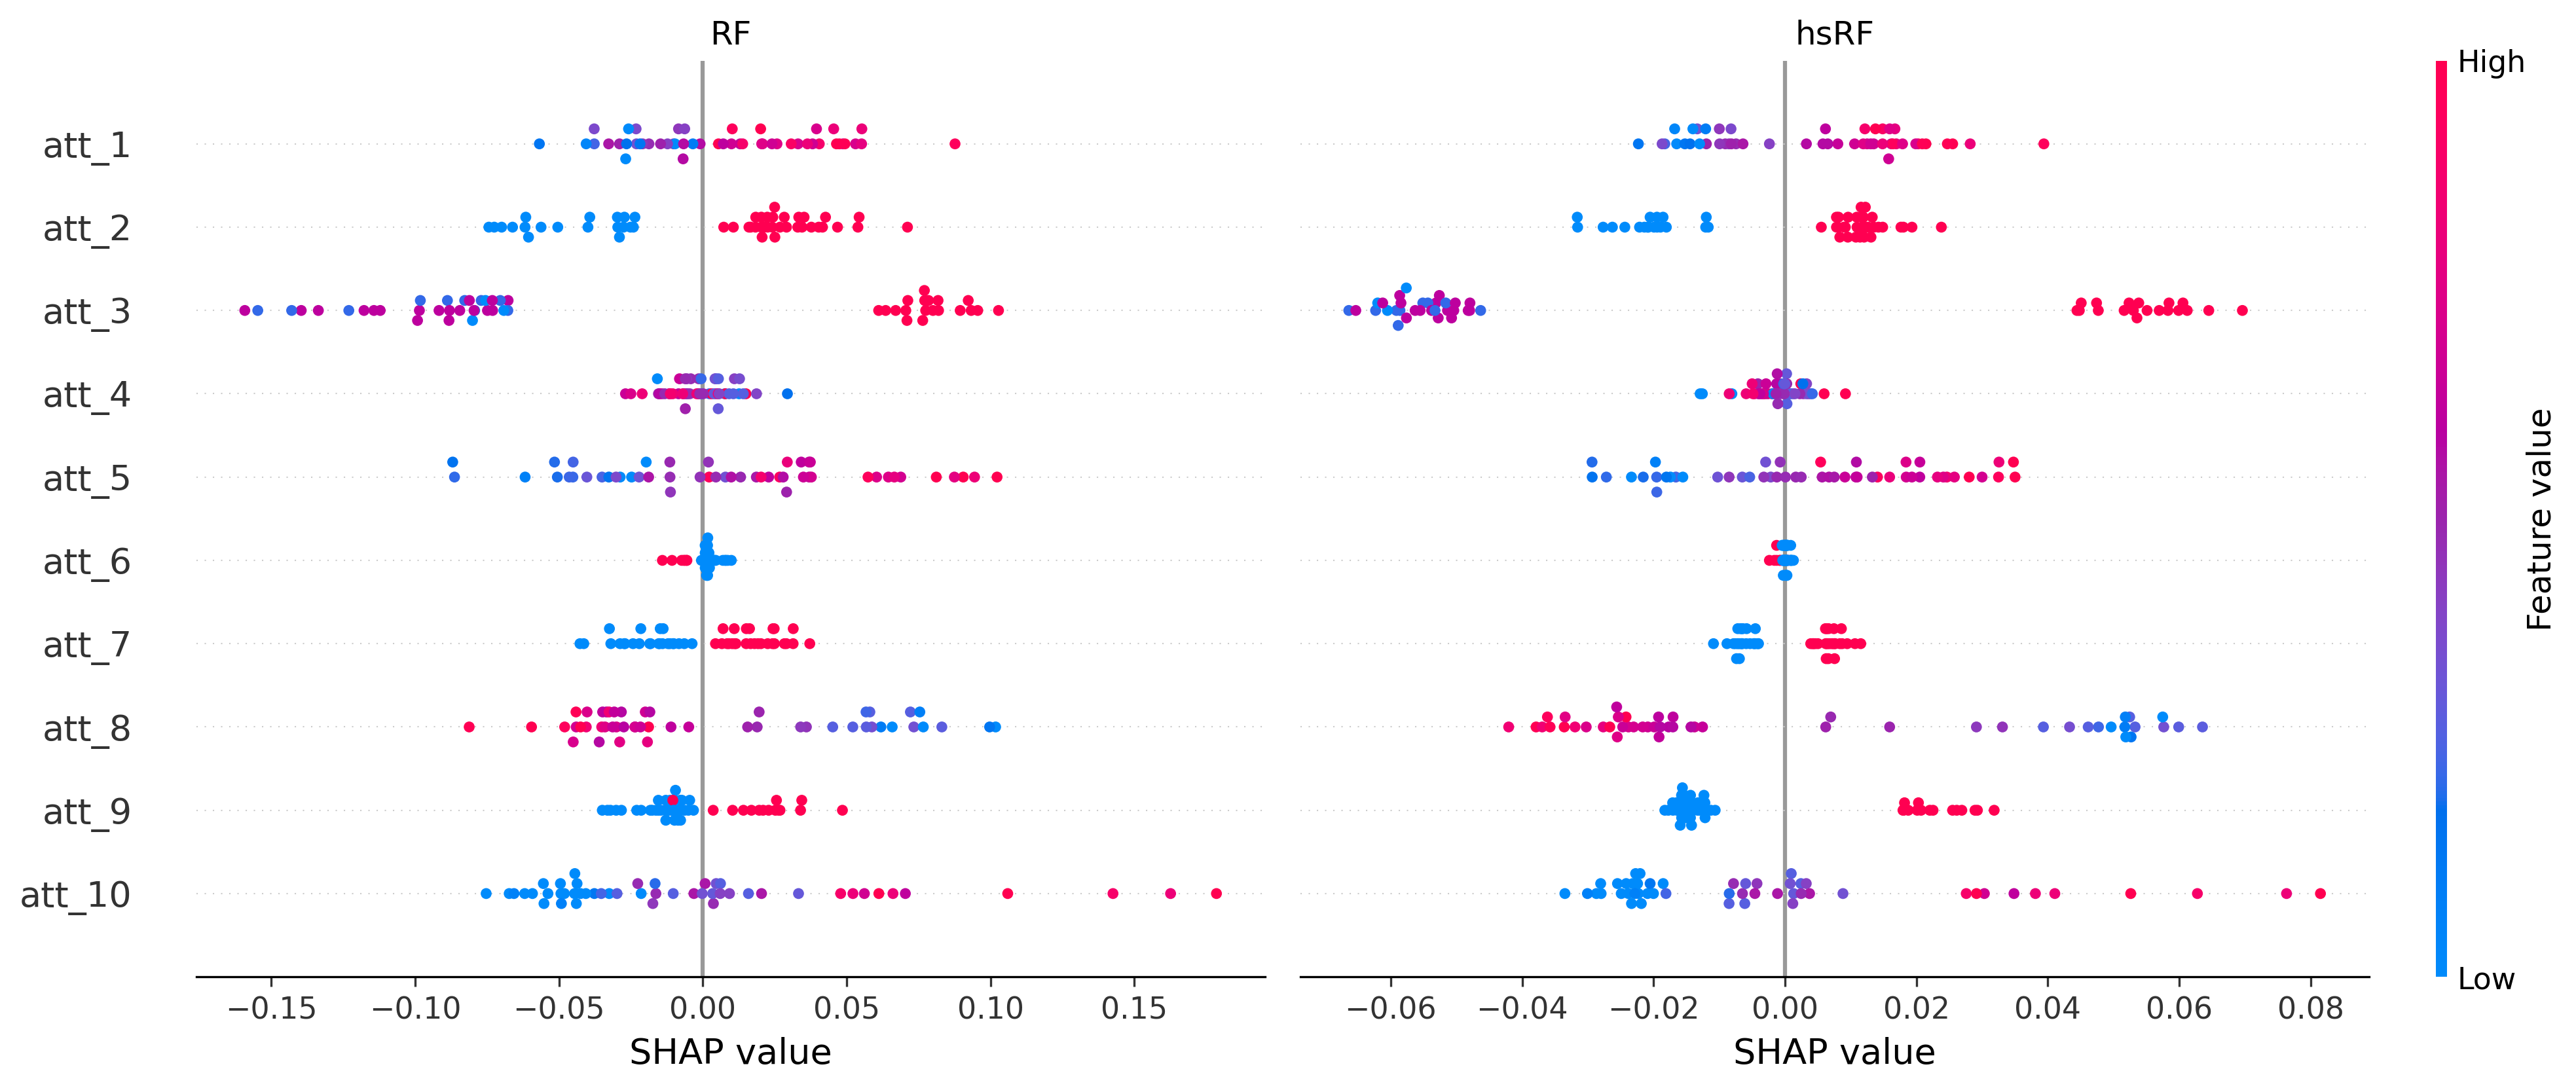
\includegraphics[width=\textwidth]{images/SHAP/shap.png}
        \caption{SHAP values for Heart dataset.}
        \label{fig:scluster}
    \end{subfigure}
    \caption{SHAP values before and after applying HS. In the upper figure (\ref{fig:svar}) we have the variance reduction for the Diabetes dataset. In the lower figure (\ref{fig:scluster}) we have the SHAP values for the Heart dataset. We can see that after applying HS (right) the SHAP values are clustered, which makes features easier to interpret.}
    \label{fig:claim4-shap}
\end{figure}

\section{Discussion}

In this report, we managed to show that HS, as a regularization technique, consistently improves DT scores. HS was also on average the best regularizer for DT. 
For RF, HS did not perform better than other regularization methods and did not consistently improve RF, however, it was significantly faster compared to other regularization methods.
We hypothesize that the divergence between our observed (Appendix~\ref{appendix:claim1},~\ref{appendix:claim2}) and the original paper scores are likely because the differences between our TBM scores were smaller.
We assume that for $mtry$ and $d_{max}$ the differences might have been caused by using a different HPS space, possibly indicating a poor choice of HPS space on the author's part, while in the instance of $RF$ our differences might be pure chance since the authors used only 10 samples for their experiments, therefore some variance in score distributions is expected.
The decision boundaries for RF were less fragmented after applying HS, which made them easier to interpret. HS also lowered SHAP value variability, and as a result, HS-RF generated more stable explanations. 
Based on our results we conclude that HS is one of the best (evaluated) regularization methods for DT in terms of all three aspects (score, speed, interpretability).
For RF, HS as a regularization method only stood out in terms of speed, scoring similarly to other regularization methods.
We also note that our results did show that HS improved interpretability, however, no comparison was done with other regularization methods.

\subsection{What was easy}

It was easy to use HS and other TBM that were implemented in the {\sf imodels} library.
The library used the same naming conventions as the {\sf scikit-learn} library, implementing most of the standard {\sf fit()}, {\sf predict()} and {\sf predict\_proba()} functions.
Furthermore, the {\sf imodels} library provides a {\sf get\_clean\_datasets()} function from which we were able to download already pre-processed datasets, allowing us to focus more of our effort on the reproduction.

\subsection{What was difficult}

Parts that required changes to the code or that were not present in the {\sf imodels} library were generally problematic to implement.
While the article did link to the paper repository the tutorial notebooks did not run out of the box and required significant modification to run.
One methodological problem was the usage of number of leaves during evaluation in spite of the fact that a number of leaves was not a hyperparameter in any of the methods implemented in either {\sf imodels} or {\sf scikit-learn}.
We concluded that the authors most likely specified the maximum number of leaves a tree could have, but we were unable to verify whether the authors used the max. number of leaves or the number of non-leaf nodes (a model attribute implemented for most TBM in the {\sf imodels} library) for evaluation. 
This was because the code in the notebooks used the latter for evaluation, while the original paper claimed to use the prior.

Another problem we encountered was that the authors did not specify how they performed hyperparameter search for methods such as $mtry$ and $d_{max}$. % and BART.
%In the instance of BART specifically, the authors only used one value for all different numbers of trees,  without specifying what this value meant or how it was calculated.

\subsection{Communication with original authors}

We did not contact the original authors. Most of the choices in the original paper were well documented and we were generally able to fill in the gaps for missing specifications based on the contents of the corresponding claim.
Additionally, we also considered not contacting the authors to have specific benefits such as using improved evaluation methodology or using different HPS techniques, which allowed us to test the robustness of the author's claims to small alterations in the proposed methodology. 
By taking this approach while our reproducibility might have possibly suffered it enabled us to expand on the authors' results in certain areas.
